Nesta seção é apresentado em detalhes a implementação aplicadas no \textit{benchmark} Bench4Q. A Figura \ref{fig:diagrama-classes} mostra o diagrama de classes envolvido na extensão do Bench4Q. As classes sinalizadas na core azul, representa as já existentes mas que passaram por adaptações e modificações, já as classes na cor verde, se refere as novas classes criadas para possibilitar a modulação da carga do \textit{benchmark}.

Apesar de permitir a geração de carga para o sistema, o Bench4Q possui algumas limitações na sua versão original que dificultam a experimentação e analise de cenários de interesse ao trabalhos de Choquehuanca e \cite{Lourenco2015} de quem pretende desenvolver técnicas de gerenciamento de recursos.
As classes disponíveis no \textit{benchmark} original não permitem a modulação de carga de trabalho, essa limitação implica, por exemplo, na dificuldade de projetar um controlador para o gerenciamento de recursos, pois para esta atividade é necessário uma análise de resultados transiente mediante a modulação da carga de trabalho, a simulação de um uma carga de trabalho em que há a alteração introduzida ao longo da simulação é o foco deste trabalho.
Para distribuir a submissão da carga de trabalho ao longo da simulação, uma estratégia utilizada é a modulação da mesma atrás de parâmetros que configuram o comportamento da carga. O Bench4Q também não suporta nativamente a alocação e a deslocação dos recursos em tempo de simulação, uma conjunto de implementações foram necessárias para estender o \textit{benchmark}, essas aplicações não lidam com a modulação da carga de trabalho, mas manipulação a distribuição da carga de trabalho em um conjunto de servidores, da mesma maneira que um ambiente de nuvem, assim como o gerenciamento dos recursos da proposta de arquitetura. Contudo, os detalhes dessa implementação não serão apresentados e discutido neste trabalho, uma vez este contexto foge do foco e da proposta do trabalho que tem como a modulação da carga.

\begin{figure}[htb]
	\centering
	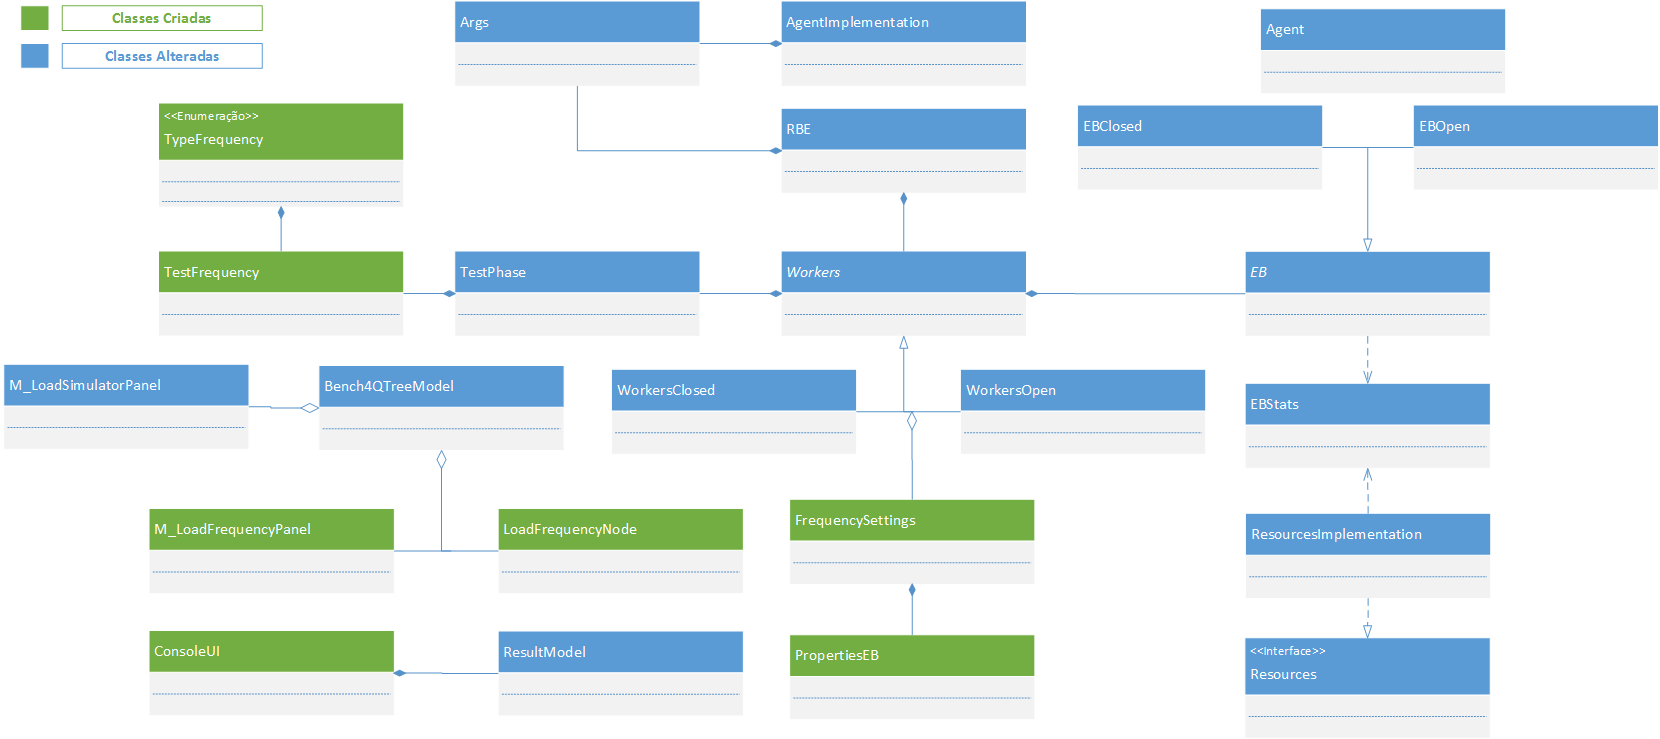
\includegraphics[scale=0.4]{diagrama-classes-beanch4Q.png}	
	\caption{Diagrama de classes da extensão do Bench4Q.}
	\label{fig:diagrama-classes}
	\fautor
\end{figure}

%1º  - falar como foi implementados as modificações conforme a metodologia

A princípio foi identificado o modulo de geração de carga do Bench4Q e este passou por alterações para gerar a carga de trabalho esperada. Conforme o diagrama de classes na figura \ref{fig:diagrama-classes}, é possível ter uma ideia do trabalho de extensão realizado no \textit{benchmark}, vale aqui salientar que o Bench4Q é uma ferramenta completa e extensa, e diagramar todas as classes do mesmo ficaria difícil e aumentaria consideravelmente a complexidade de entendimento da mesma, sendo assim, aqui apresentamos somente as classes já existente no Bench4Q e que passar por modificações para atender aos requisitos da metodologia, juntamente com as novas classes que foram necessária para almejar o mesmo objetivo.

O Bench4Q fornece uma estrutura e componentes compartilhados para a comunicação entre os dois módulos da carga de trabalho, \textbf{Console} e \textbf{Agente}. Apesar de trabalharem em conjunto e para um mesmo fim, cada modulo (Console e Agente) são executados em máquinas distintas.  A extensão é construída inicialmente sob a classe \textsf{MLoadSimulatorPanel}, que orquestra toda a interatividade gráfica do Bench4Q. O novo painel de configuração, que modula a carga, \textsf{MLoadFrequencyPanel} estende da classe original \textsf{Bench4QTreeModel}, adicionando os parâmetros para a modulação: tipo da carga, o instante em que a carga se inicia, o tempo de atuação da carga e a quantidade de EBs que atuaram nessa carga. O parâmetro \textit{"tipos de carga"}, utiliza da classe enum \textsf{TypeFrequency} que define as constantes dos tipos de modulações programadas para esta extensão.  Todos os parâmetros inseridos na \textsf{MLoadSimulatorPanel} são armazenados na classe \textsf{TestFrequency} que se tornou um propriedade da classe nativa \textsf{TestPhase}, que posteriormente são repassadas para a classe \textsf{PropertiesEB} através da \textsf{FrequencySettings}. Já nas classes \textsf{Agent}, \textsf{EB}, \textsf{EBClose}, \textsf{EBOpen}, \textsf{Workers}, \textsf{WorkersClosed} e \textsf{WorkersOpen} foram modificadas para receber os novos parâmetros da \textsf{PropertiesEB} e compreendê-los correspondentemente a modulação configurada na interface gráfica e gerando a carga programada durante a execução.

Este conjunto de classes as quais lidam, manipulam, gerenciam e modulam a carga de trabalha gerada pelo Bench4Q, utilizam de um excelente console para configurar, monitorar e analisar todo o experimento. Todo o desenvolvimento, referente à modificação e implementação de novas classes, mantiveram e respeitaram o padrão de desenvolvimento do \textit{benchmark}. A figura \ref{fig:interface-criada-beanch4q} ilustra a interface gráfica por onde é possível modular a carga de trabalho do Bench4Q. 

\begin{figure}[htb]
	\centering
	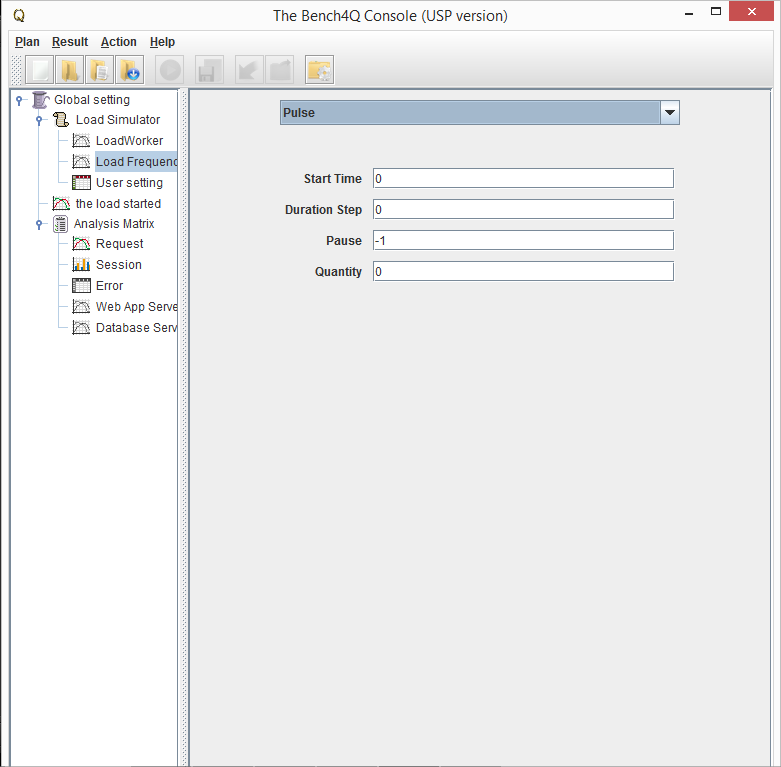
\includegraphics[scale=0.6
	]{console-bench4Q-usp.png}
	\caption{Console de programação de carga de trabalho.}
	\label{fig:interface-criada-beanch4q}
	\fautor
\end{figure}

Informar previamente a execução os parâmetros da modulação, como por exemplo, ao escolher a opção degrau, é necessário informar quantos EBs geram o degrau, em que instante de tempo, e qual o tempo de duração e por fim qual a sua polaridade (com base em um pulso elétrico a positiva sairia de zero e chega a um, a negativa, sairia de um e chegaria a zero), é possível obter resultados conforme a figura \ref{fig:grafico-carga-modulada-teste}.

\begin{figure}[!htb]
	\centering
	\begin{subfigure}{\linewidth}
		\centering
		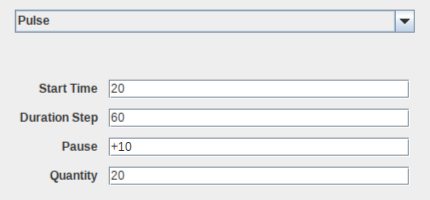
\includegraphics[scale=0.7]{condiguracao-carga-modulada1.png}
		\caption{Teste de configuração da carga a ser modulada}
		\label{fig:configuracao-carga-modulada-teste}
	\end{subfigure}
	
	\begin{subfigure}{\linewidth}
		\centering
		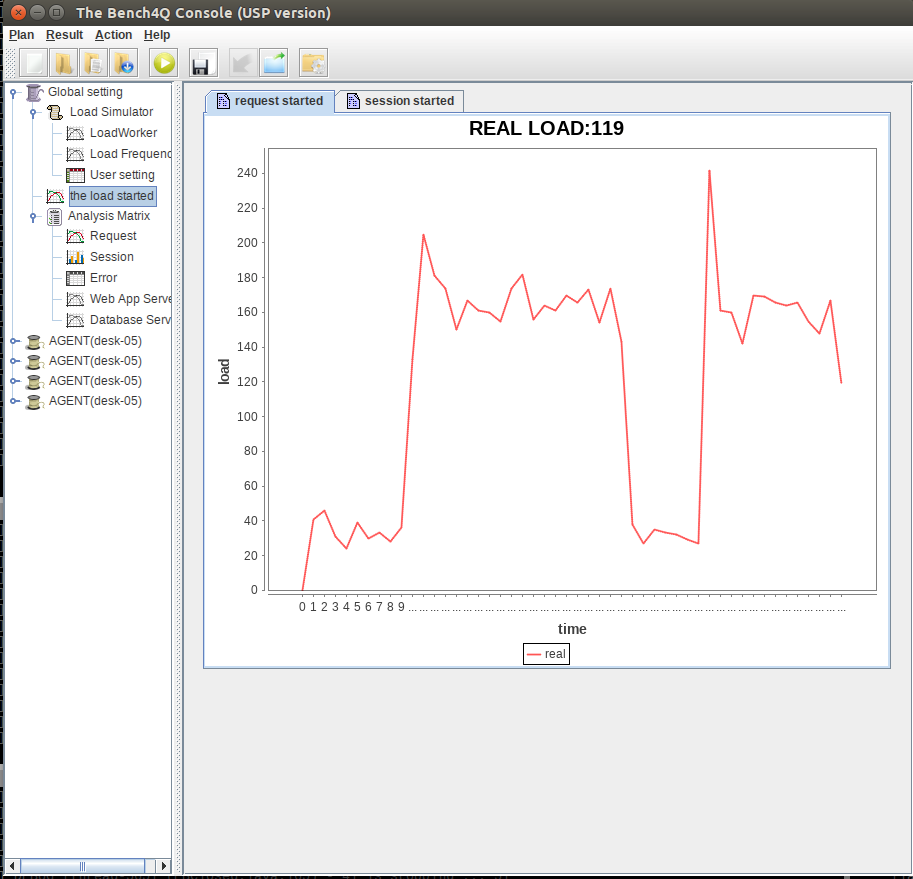
\includegraphics[scale=0.6]{grafico-carga-modulada-teste.png}
		\caption{Carga gerada com base na configuração teste}
		\label{fig:grafico-carga-modulada-teste}
	\end{subfigure}  
	\caption{Teste de modulação da carga}  
	\label{fig:carga-modulada-teste}
	\fautor
\end{figure}  

A carga de trabalho é imposta ao sistema por meio de requisições HTTP enviadas pelos EBs (usuários finais) ao SUT (serviço Web) que são executadas nos servidores de aplicação das máquinas virtuais instanciadas no \textit{host}. Essas requisições exigem que as máquinas virtuais se ocupem pelo tempo necessário para processá-las, alterando o desempenho experimentado pelo sistema.
Segundo \cite{Nobile2013}, dois fatores que envolvem uma requisição e que afetam diretamente o desempenho do sistema:
\begin{citacao}
	o tempo de processamento e a quantidade de carga imposta pelas requisições, dados pelo tempo de processamento e pela taxa de chegada de novas requisições, respectivamente. Com o tempo, a quantidade e o tamanho das requisições podem se alterar, dependendo do perfil de utilização dos usuários que utilizam o serviço naquele momento. Havendo um aumento em algum desses fatores é possível que o desempenho do sistema sofra degradação, podendo, e casos extremos, entrar em colapso.
\end{citacao}
%- ilustrar com os graficos do proprio bench4Q

A figura \ref{fig:carga-modulada-teste} ilustra uma carga teste modulado já pela extensão, na \ref{fig:configuracao-carga-modulada-teste} apresenta os parâmetro utilizado para fazer o teste, a carga modulada atuará a partir do 10º segundo de experimentação e com uma duração de 20 segundos, com 30 segundo de experimentação ocorrerá uma pausa de 7 segundos e um novo degrau será gerado em seguida, que se manterá até o final do experimento. Para este exemplo fora fixados 40 EBs para modulara o comportamento da carga. Este comportamento pode ser apreciado no item \ref{fig:grafico-carga-modulada-teste} da mesma figura \ref{fig:carga-modulada-teste}. Vale salientar que o gráfico gerado e apresentado na figura \ref{fig:carga-modulada-teste} de item \ref{fig:grafico-carga-modulada-teste}, é uma característica nativa ao \textit{benchmark}.